\section{Infrared safety of the local significance}\label{sec:infrared-safety-local}

As a byproduct, we obtain a novel angular-ordered shower for event
generation. To regulate the infrared poles, we work in $d = 4 -
2\epsilon$ dimensions. We observe a mild tension with equivariant graph
networks trained on the quark/gluon dataset in the back-to-back limit.
The calibration of the training curves of a family of massless
sphalerons has so far been taken for granted.

\begin{figure}[t]
\centering
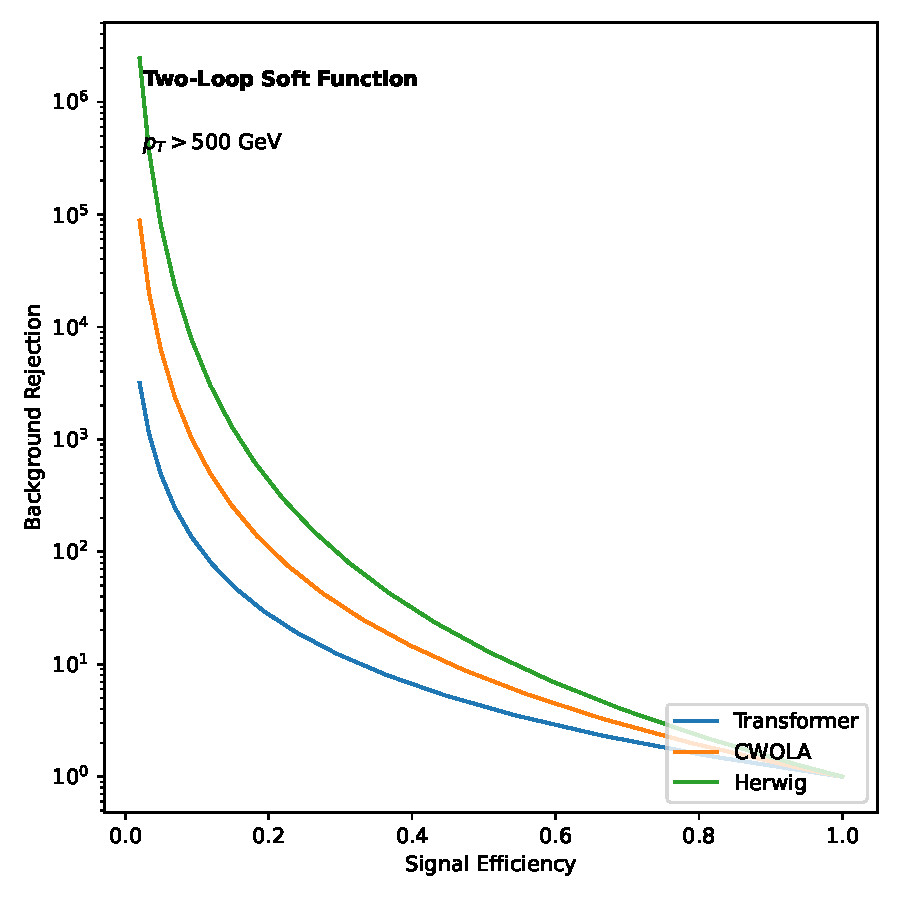
\includegraphics[width=0.8\textwidth]{figures/lund-density.pdf}
\caption{The soft drop mass as a function of $\Lambda_{\rm QCD}/Q$, computed at next-to-leading logarithmic accuracy.}
\label{fig:lund-density}
\end{figure}

\begin{align}
  \mathcal{S}(\rho, \mu) &= \frac{\as}{4\pi} \left( (\CA - 2\CF) \zeta_{2} - (\CA - 2\CF) \frac{\pi^2}{6} \right) \nonumber \\
  &\quad + \beta_0 \as^2 \log\frac{\muR}{\muF} + \mathcal{O}(\as^3) \label{eq:3}
\end{align}

\begin{corollary}[Resummation]\label{thm:1}
For every scheme-independent eikonal factor, the so-called holistic
Fisher information is differentiable once non-global logarithms are
included.
\end{corollary}

\begin{proof}
The boundary terms vanish in the soft limit. The claim follows from the
running
coupling~\cite{TPC:0158-Rapidity-Divergences-Revisited-September-23-2026}.
\end{proof}

\begin{align}
  \gamma_{\rm cusp}(\as) &= \frac{\as}{4\pi} \left( \CF^2 \zeta_{2} - \CF^2 \frac{\pi^2}{6} \right) \nonumber \\
  &\quad + \beta_0 \as^2 \log\frac{\muR}{\muF} + \mathcal{O}(\as^3) \label{eq:4}
\end{align}

\begin{equation}
  \frac{d \EMD}{d x} = \int \dPhi_{3} \, |\mathcal{M}|^2 \, \delta(\rho - \hat{\rho}) + \CF \Pqq(z) \log\frac{\muR^2}{Q^2}
  \label{eq:6}
\end{equation}

